\begin{figure}[!h]
    \centering
    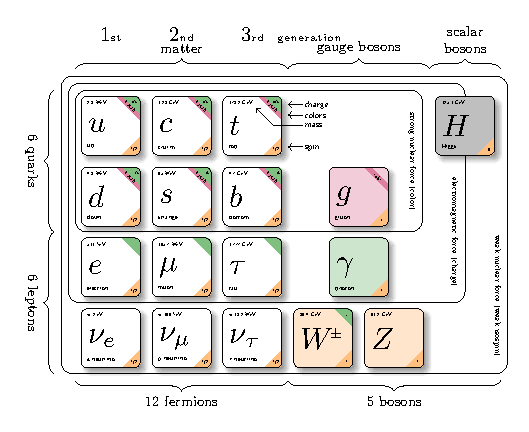
\includegraphics[width=0.95\textwidth]{figures/SM_figure.pdf}
\end{figure}
\section{The Standard Model}\label{ch:SM}
In order to describe the three quantizable forces of nature, we gather the mediators of each force -- the vector bosons -- into local (gauge) symmetry groups. 
Each vector boson has one corresponding generator, the set of which constitutes the group.
The strong charge is mediated by eight massless gluons, which correspond to the eight independent generators of $\text{SU}(3)_C$. 
The weak charge is mediated by the three massive gauge bosons $W^\pm$ and $Z$, and the massless photon $\gamma$, 
which constitute the generators of $\text{SU}(2)_L$ and $\text{U}(1)_Y$. 

The subscript of each group denotes by which mechanism that force is mediated. The gluons mediate the strong force through interactions of color,
emphasized with subscript $C$. The weak force only sees left-handed particles, 
which we distinguish with the subscript $L$. And the electroweak interaction that a particle undergoes is determined by its hypercharge $Y$. 
For example, the quarks all have a non-zero color and non-zero hypercharge, 
so they participate in the strong and electromagnetic interactions. If a quark is left-handed, it will also feel the weak interaction. 
The neutrinos, on the other hand, have neither charge nor color, 
so they are invisible to both the strong and electromagnetic force. We express this by letting their fields transform as singlets under those symmetry groups.

\subsection{Beyond the Standard Model}
Together, these three interactions make up the Standard Model gauge group $\mathrm{SU}(3)_{\mathrm{C}} \times \mathrm{SU}(2)_{L} \times \mathrm{U}(1)_{Y}$. 
This determines the form of the three coupling constants, which numerical values must be experimentally measured. 
Since the vector bosons are represented by the generators, they are uniquely determined by the symmetry group. However, the scalar boson(s) and fermions are free as long as they
belong to representations of the symmetry group. By this construction, modifications to fermions rather than bosons are generally easier to make, allowing us to propose amendments to the model. Even the
number of fermions must be experimentally verified and can be altered from a phenomenological standpoint. In this work,
we will use this leniency to introduce a new particle and examine to which extent 
these modifications might be supported by experimental evidence. Moreover, we will examine the possibility of adding a new completely new interaction, which manifests itself as modifications to the neutrino-matter interactions.

\section{Mass Generation}
In the Standard Model, fermion masses are generated by the Higgs mechanism through Yukawa couplings with the fermion's right and left-handed components.
All neutrinos are left-handed, and all antineutrinos are right-handed~\cite{giunti}. This observational fact is reflected in the 
left-handed lepton doublet and right-handed lepton singlet

\begin{align}
    L^\prime_{\alpha L} = \begin{pmatrix}
            \nu^\prime_{\alpha L} \\
        \alpha^\prime_{L} 
    \end{pmatrix}\,, \quad
    \ell^\prime_{\alpha R} =
    \alpha^\prime_{R} \,,            
\end{align}
where $\alpha \in \{e,\mu,\tau\}$, and the primes denotes that the fields do not have definite masses.
The essential part here is that $\nu^\prime_{\alpha R}$ is missing from the right-handed lepton singlet.
Thus, the neutrino fields do not pick up a Yukawa coupling, 
and will not undergo the Higgs mechanism, which leaves them massless.
Moreover, all terms of a Lagrangian that we construct must respect the gauge invariance. This removes the possibility of the neutrino mass to be 
generated at loop level because any such attempt will violate the total lepton number by two units.
In order to keep our theory renormalizable, we have one option left if we want to generate neutrino masses: introducing right-handed neutrino and left-handed antineutrino fields. 

We consider a right-handed neutrino field, $\nu^\prime_R$. Since the electroweak gauge group $\text{SU}(2)_L \times U(1)_Y$ only couple to 
left-handed particles and right-handed antiparticles, $\nu_R$ transforms as a singlet under the Standard Model symmetry 
group $\mathrm{SU}(3)_{\mathrm{C}} \times \mathrm{SU}(2)_{L} \times \mathrm{U}(1)_{Y}$. 

We extend the Standard Model by adding a right-handed component of this field with neutrino Yukawa couplings $Y_{\alpha \beta}^{\prime \nu}$ to the Higgs-lepton Yukawa part of the interaction Lagrangian 
\begin{align} 
    \mathcal{L}_{int} \subseteq -\left( \frac{v + H}{\sqrt{2}} \right) \left[ \bar{\ell}^{\prime}_{\alpha L} Y_{\alpha \beta}^{\prime \ell} \ell_{\beta R}^{\prime} + \bar{\nu}_{\alpha L}^{\prime} Y_{\alpha \beta}^{\prime \nu} \nu_{\beta R}^{\prime}\right]\,,
\end{align}
where $v$ is the Higgs vacuum expectation value, $H$ the Higgs field, $\ell_{\alpha L}^\prime (\ell_{\beta R}^\prime)$ the left (right) handed charged lepton field, and summation over the lepton indices $\alpha,\beta$ is implied. $Y_{\alpha \beta}^{\prime \ell}$ are the charged lepton Yukawa couplings, and $\nu^\prime_{\alpha L}(\nu^\prime_{\beta R})$ are the left (right) handed neutrino fields .
Now, the Yukawa coupling matrices $Y^{\prime \ell}$ and $Y^{\prime \nu}$ are non-diagonal, as emphasized with their prime. 
This can be remedied by diagonalizing $Y^{\prime \ell}$  with a biunitary transformation
\begin{align}
    V_{ L}^{\ell \dagger} Y^{\prime \ell} V_{ R}^{\ell}=Y^{\ell} \,.
\end{align}
where $V^\ell_L$ and $V^\ell_R$ are two unitary matrices.
Similarly, we diagonalize and $Y^{\prime \nu}$ with a unitary matrix $V^\nu$. 
Now we state a crucial difference between the properties of the charged lepton and the neutrino fields.
While the charged lepton flavor eigenstate was uniquely determined by its mass eigenstate, the neutrino flavor is a superposition of mass eigenstates. 
This is because neutrinos are indirectly detected via the observation of its associated charged lepton, so there is no requirement for neutrino flavor eigenstates to have a definite mass. 
The flavor of a neutrino is then -- by definition -- the flavor of the associated charged lepton. 
This fact is denoted as giving the mass eigenstates Latin numerals and letters, while the flavor eigenstates stay as Greek letters.

So, let the neutrino field in the mass basis have components with Latin numerals to distinguish them from the flavour components, i.e 
\begin{align}\label{eq:nu_rotation} 
    \nu_{k} =  V_{k\beta}^{\nu \dagger} \nu_{\beta}^\prime\,.
\end{align}
The diagonalized Lagrangian now takes the form 
\begin{align}
    \mathcal{L}_{int} &\subseteq -\left( \frac{v + H}{\sqrt{2}} \right) \left[\bar{\ell}_{\alpha L}^{\prime} Y_{\alpha \beta}^{\prime \ell} \ell_{\beta R}^{\prime} + \bar{\nu}_{\alpha L}^{\prime} Y_{\alpha \beta}^{\prime \nu} \nu_{\beta R}^{\prime}\right] \nonumber \\
    &= -\left( \frac{v + H}{\sqrt{2}} \right) \left[\bar{\ell}_{\alpha L}^{\prime} V_{\alpha \beta L}^{\ell} Y_{\alpha \beta}^{ \ell} V_{\alpha \beta R}^{\ell \dagger} \ell_{\beta R}^{\prime}
    + \bar{\nu}_{\alpha L}^{\prime} V_{\alpha k L}^{\nu} Y_{kj}^{\nu} V_{\beta j  R}^{\nu \dagger} \nu_{\beta R}^{\prime}\right] \nonumber \\
    &= -\left( \frac{v + H}{\sqrt{2}} \right) \left[\bar{\ell}_{\alpha L} Y_{\alpha \beta}^{ \ell} \ell_{\beta R} + \bar{\nu}_{k L} Y_{kj}^{ \nu} \nu_{j R}\right] \nonumber \\
    &= -\left( \frac{v + H}{\sqrt{2}} \right) \left[\bar{\ell}_{\alpha L} Y_{\alpha \beta}^{ \ell} \ell_{\beta R} + \bar{\nu}_{k L} Y_{kj}^\nu \nu_{j R}\right]
\end{align}
By construction, $Y^\ell$ and $Y^\nu$ are diagonal, so we write their components as $y_{\alpha}^{\ell} \delta_{\alpha \beta}$ and $y_{k}^{\nu} \delta_{k j}$ respectively, leaving the Lagrangian as 
\begin{align}\label{eq:L_H}
    \mathcal{L}_{int} 
    &\subseteq-\left( \frac{v + H}{\sqrt{2}} \right) \left[\bar{\ell}_{\alpha L} y_{\alpha}^{\ell} \delta_{\alpha \beta} \ell_{\beta R} + \bar{\nu}_{k L} y_{k}^{\nu} \delta_{k j} \nu_{j R}\right] \nonumber \\
    &=-\left( \frac{v + H}{\sqrt{2}} \right) \left[\bar{\ell}_{\alpha L} y_{\alpha}^{\ell}  \ell_{\alpha R} + \bar{\nu}_{k L} y_{k}^{\nu} \nu_{k R}\right] \nonumber \\
    &=-\left( \frac{v + H}{\sqrt{2}} \right) \left[ y_{\alpha}^{\ell}  \bar{\ell}_{\alpha L}\ell_{\alpha R} +  y_{k}^{\nu}\bar{\nu}_{k L} \nu_{k R}\right] 
\end{align}
Now, by the introduction of the right-handed field $\nu_R$, the Dirac neutrino field is
\begin{align}
    \nu_k = \nu_{kL} + \nu_{kR}\,.
\end{align}
Multiplying $\nu_k$ with its conjugate $\bar{\nu}_k$, we get 
\begin{align}
    \bar{\nu}_k \nu_k 
    & = \bar{\nu}_{k L} \nu_{k L} +\bar{\nu}_{k R}\nu_{k L} + \bar{\nu}_{k L}\nu_{k R} + \bar{\nu}_{k R}\nu_{k R} \nonumber \\
    & = \bar{\nu}_{k L}\nu_{k R} + \bar{\nu}_{k R}\nu_{k L} \nonumber \\
    & = \bar{\nu}_{k L}\nu_{k R} + \t{h.c.}
\end{align}
The same calculation for the charged lepton field yields the same result for $\ell_k$. Substituting this result and multiplying the Higgs vacuum expectation value $v$ into the fields gives us
\begin{align}
    \mathcal{L}_{H} 
    &=-\left( \frac{v + H}{\sqrt{2}} \right) \left[ y_{\alpha}^{\ell}   \bar{\ell}_\alpha \ell_\alpha  +  y_{k}^{\nu} \bar{\nu}_k \nu_k \right] \nonumber \\
    &=- \frac{y_{\alpha}^{\ell} v}{\sqrt{2}}   \bar{\ell}_\alpha \ell_\alpha   -  \frac{ y_{k}^{\nu} v}{\sqrt{2}} \bar{\nu}_k \nu_k  - \frac{y_{\alpha}^{\ell}}{\sqrt{2}}   \bar{\ell}_\alpha \ell_\alpha H  -  \frac{ y_{k}^{\nu}}{\sqrt{2}} \bar{\nu}_k \nu_k H\,.
\end{align}
Thus, this extension to the SM generates by the Higgs mechanism neutrino masses with terms
\begin{align}
    m_k = \frac{y_k^\nu v}{\sqrt{2}}\,,
\end{align}
where the Yukawa couplings $y^\nu_k$ needs to be experimentally determined.